\begin{outline-text-1}
\begin{xlarge}
\begin{center}
To Start Press "n"
\end{center}
\end{xlarge}

\begin{center}
\textbf{WARN} Turn off your custom keyboard shortcuts
\end{center}

\begin{note}
\begin{alignright}
Made by guicho2.71828 (Masataro Asai)
\end{alignright}
\end{note}
\end{outline-text-1}

\section{What Is It?}
\label{sec-1}

\begin{xlarge}
An Alternative to
\begin{center}
Org-based Presentation
\end{center}
\begin{alignright}
Method
\end{alignright}
\end{xlarge}

\begin{center}
Proceed with "n"
\end{center}
\section{Usage (on browsers)}
\label{sec-2}

\begin{smaller}
\begin{description}
\item[{n}] go to the next section/expand a list
\item[{p}] back to the previous section
\item[{s, or "go"}] jump to an arbitrary section (using minibuffer)
\item[{d}] debugging mode (shows content border)
\item[{<Ctrl-g> or <Esc>}] cancel current key strokes
\item[{"help"}] shows the available commands in the minibuffer!
\end{description}
\end{smaller}
\section{Usage (on emacs)}
\label{sec-3}

\begin{enumerate}
\item clone \href{https://github.com/guicho271828/another-org-info}{our repo}

\item \texttt{make} to publish

\item show it on your browser!
\end{enumerate}
\section{Virtue}
\label{sec-4}

\begin{itemize}
\item Simplicity
\begin{itemize}
\item \texttt{code.js} only has 200 lines
\end{itemize}
\item Extensibility
\begin{itemize}
\item you can write your own extension and its easy
\item set a function to \texttt{keyManager.<your-key-strokes>}
\item any char code \(c\) in the keystrokes must be \(32 < c < 126\)
\begin{itemize}
\item \texttt{Space,!,",...A,B,C,...x,y,z,\{,|,\textasciitilde{}}
\end{itemize}
\end{itemize}
\item LICENSE
\begin{itemize}
\item GPLv3 ?? < not attatched a lisence yet
\end{itemize}
\end{itemize}
\section{Example: Expanding a List}
\label{sec-5}

\begin{itemize}
\item \textbf{the dots} tell "\emph{here are more contents}" \(\rightarrow\)
\item \textbf{an arrow} tells "\emph{here are expandable contents}" \(\rightarrow\)
\begin{itemize}
\item These remind you that there are
\item \textbf{still more sub-contents} you have to talk
\item and where it ends
\end{itemize}
\item list
\item list
\end{itemize}
\section{Org-block templates}
\label{sec-6}

\texttt{another-org-info} knows are:

\begin{itemize}
\item <S -- smaller
\item <lar -- larger
\item <t -- twocolumn
\begin{itemize}
\item implemented using a part of CSS in \href{http://getbootstrap.com/}{twitter-bootstrap}
\end{itemize}
\item <n -- footnote
\item <r -- float right
\item <ar -- align right
\item <lcr -- "left,center,right" format with x-large fonts
\item <E -- latex `equation' environment
\item still more\ldots{}
\end{itemize}

\subsection{copy-paste it}
\label{sec-6-1}

to your \texttt{.emacs}

\begin{center}
\url{config.el}
\end{center}
\section{Dependency}
\label{sec-7}
\label{dependency}

\begin{itemize}
\item jQuery 1.10.2 (included)
\item org-mode v8.1 (not presicely)
\end{itemize}

\subsection{Utility}
\label{sec-7-1}

\begin{itemize}
\item ./make-periotically.sh [args]
\begin{itemize}
\item Watches the changes in the directory and \texttt{make}
\item A simple shell script
\item all arguments are passed to \texttt{make}
\item dependency : inotifywait, notify-send
\end{itemize}
\end{itemize}
\section{Test}
\label{sec-8}

\begin{itemize}
\item \href{http://www.google.com}{Link}
\item This
\item Is
\item A Test
\end{itemize}

Mathjax formula:

\[
 E=mc^2
\]

\begin{equation}
 E=mc^2 + \frac{1}{2} mv^2
\end{equation}

\subsection{Twocolumn Test}
\label{sec-8-1}

\begin{container-fluid}
\begin{row-fluid}
\begin{span6}
\begin{itemize}
\item HOOA!
\item \textbf{HOOA!}
\item HOOA!
\end{itemize}
\end{span6}
\begin{span6}
This is a LISP ALIEN IN A CAGE!

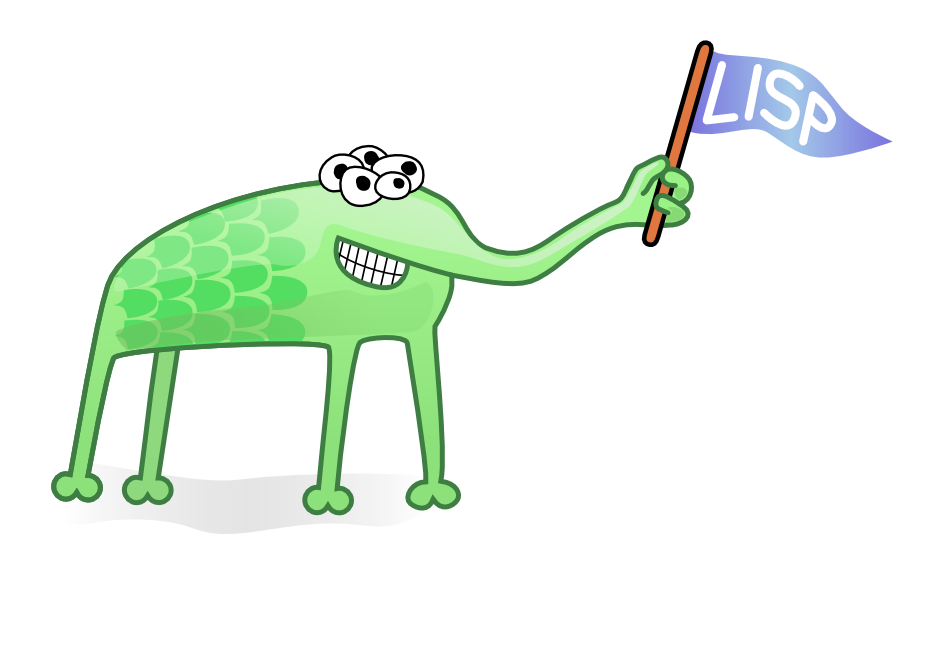
\includegraphics[width=.9\linewidth]{img/alien.png}
\end{span6}
\end{row-fluid}
\end{container-fluid}
\subsection{many columns test}
\label{sec-8-2}


\begin{container-fluid}
\begin{row-fluid}
\begin{span3}
a a a a a a a a a a a a a a a a a a a a a a a a a a a a a a a a
\end{span3}
\begin{span3}
b b b b b b b b b b b b b b b b b b b b b b b b b b b b b b b b
\end{span3}
\begin{span3}
c c c c c c c c c c c c c c c c c c c c c c c c c c c c c c c c
\end{span3}
\begin{span3}
d d d d d d d d d d d d d d d d d d d d d d d d d d d d d d d d
\end{span3}
\end{row-fluid}
\end{container-fluid}

\section{A Slide with Too Little Contents}
\label{sec-9}

\begin{center}
\begin{smaller}
Hi, I'm small!
\end{smaller}
\end{center}

\begin{note}
See the headline is correctly adjusted
\end{note}
\section{Left-Center-Right template}
\label{sec-10}

\begin{xlarge}
x-large left
\begin{center}
centered
\end{center}
\begin{alignright}
right
\end{alignright}
\end{xlarge}

\begin{note}
This is a footnote
\end{note}
\section{TODOs}
\label{sec-11}


\begin{container-fluid}
\begin{row-fluid}
\begin{span6}
\begin{smaller}
\begin{itemize}
\item Features
\begin{itemize}
\item Table of contents
\item \texttt{<dl>} does not expand
\item \sout{Showing current keystrokes} \textbf{DONE}
\item auto-scroll/auto-zoom with big contents
\item Showing current/total page number
\item Changing Stylesheet
\item Up-Section command
\item Slide thumbnail
\item \sout{stopwatch/countdown timer} \textbf{DONE}
\item link to \#section
\end{itemize}
\end{itemize}
\end{smaller}
\end{span6}
\begin{span6}
\begin{smaller}
\begin{itemize}
\item Features inspired by other tools
\begin{itemize}
\item Content Search (in org-infojs)
\item Drawing mode (in \href{http://code.google.com/p/jessyink/}{jessyink})
\item 'Paused' mode (in \href{http://lab.hakim.se/reveal-js/}{reveal.js})
\item \sout{Export to PDF (also in reveal.js)}
\begin{itemize}
\item implemented as the resume output
\end{itemize}
\item Slide with an image covering entire background (slideshare)
\item present one paragraph/word/letter at a time
\begin{itemize}
\item those in \href{http://docutils.sourceforge.net/docs/user/slide-shows.s5.html}{s5}
\end{itemize}
\item "C-M-x" style notation in the command definition
\end{itemize}
\end{itemize}
\end{smaller}
\end{span6}
\end{row-fluid}
\end{container-fluid}
